
	%% setup reference database.
	\bibliography*{20131020anarticle}
	\bibliographystyle*{bibstyle}     %% setup reference style.
	%% Section title
	\section{2012年5月工作总结}
	
	%\end{abstract}
\section{热辐射热传导耦合问题的边界元方法}

本文的主要研究问题是边界热辐射与热传导耦合问题。边界热辐射现象主要出现在不透明
的固体表面之间,工程中的大部分固体材料均为不透明固体,他们只有表面很薄的一层参与热射线的吸收和发射,例如厚度为0.1$\mu m$的金,银,铂在红外波段的穿透率都小于0.003\cite{yu2000},因此这类材料的内部换热方式为热传导导热,表面间的换热方式为热辐射发射和反射换热。

固体表面的热辐射物性主要指发射率,吸收率,和反射率,这些量与热射线的波长,吸收发射方向,以及表面状态有关\cite{yu2000}。为了简化模型,常常采用参与辐射换热的表面是漫灰体的假设,即辐射表面与辐射物性参数与热射线的发射,反射,吸收方向无关,且与热射线的波长无关。

在上述假设下,边界热辐射和热传导的耦合的控制方程为
\begin{equation}
	\begin{cases}
		 c(x,t) \rho(x,t) \frac{\partial u(x,t)}{\partial t} - k \Delta u(x,t) = f,              & t\in [0,T],x\in\Omega, \\
		u(x,t) = u_0(x,t),                          & t\in [0,T],x\in\Gamma,\\
		- k \frac{\partial u(x,t)}{\partial n} = q_0(x,t), & x \in  \Sigma,\\
		- k \frac{\partial u(x,t)}{\partial n} = G(\sigma T^4(x,t)) , &x \in \Sigma_r,\\
		u(\cdot,0)=u_0, & x \in \Omega.
		\end{cases}
	\label{eq:timedepand}
\end{equation}
其中,$c$为比热,$\rho$为密度,$k$为热传导系数,$G$为按如下方式定义一个积分算子\cite{druet2010weak},
\begin{eqnarray}
	G(\sigma T^4) = (I-K)R=((I-K)(I-(I-E)K)^{-1}E)(\sigma T^4)),\label{eq:rbie} \\
	R = \varepsilon\sigma T^4 + (1-\varepsilon)K(R) = (I-(1-\varepsilon)K)^{-1}\varepsilon\sigma T^4, \\
	K(f)(s) = \int_{\Sigma}w(s,z)f(z)dz, \forall s \in \Sigma, \forall f \in L^{\infty}(\Sigma),
	\label{eqoperators}
\end{eqnarray}

上述方程组是一个非线性微分积分系统,文献\cite{druet2010weak}研究了该瞬态问题解的存在唯一性。为了研究该问题的数值算法,先研究稳态问题的数值解法,即问题

\begin{equation}
	\begin{cases}
		 - k \Delta u(x,t) = f,              &x\in\Omega, \\
		u(x) = u_0(x),                          & x\in\Gamma,\\
		- k \frac{\partial u(x)}{\partial n} = q_0(x), & x \in  \Sigma,\\
		- k \frac{\partial u(x)}{\partial n} = G(\sigma T^4(x)) , &x \in \Sigma_r.
		\end{cases}
	\label{eq:main}
\end{equation}

其中算子$G$的定义同前所述,文献\cite{modest2003}中给出了算子$G$如下式所示一种表达式,
\begin{equation}
  {q_r}(x) = \varepsilon (x)\int_{{\Gamma _r}} {\left( {\frac{1}{{\varepsilon (y)}} - 1} \right){q_r}(y)w(x,y)d\Gamma (y)}+ \sigma \varepsilon (x){T^4}(x) - \varepsilon (x)\int_{{\Gamma _r}} {\sigma {T^4}(y)w(x,y)d\Gamma (y)} , 
\end{equation}
其中$w(x,y)=w^*(x,y)\cdot \beta (x,y)$,$w^*(x,y)$为辐射角系数的核函数,$\beta (x,y)$为可视因子,它们的定义分别为
\[w*(x,y) = \left\{ {\begin{array}{*{20}{c}}
  {\frac{{\left[ {{n_x} \cdot (y - x)} \right]\left[ {{n_y} \cdot (x - y)} \right]}}{{2|x - y{|^3}}}}&{x,y \in {R^2}} \\ 
  {\frac{{\left[ {{n_x} \cdot (y - x)} \right]\left[ {{n_y} \cdot (x - y)} \right]}}{{\pi |x - y{|^4}}}}&{x,y \in {R^3}} 
\end{array}} \right.\]
\[\beta (x,y) = \left\{ {\begin{array}{*{20}{c}}
  1&{\overline {xy}  \cap \Omega  = \Phi } \\ 
  0&{\overline {xy}  \cap \Omega  \ne \Phi } 
\end{array}} \right.\]
这个方程是关于辐射净热流密度的方程。

还有一种辐射方程的通过中间变量有效辐射描述方式。参考文献\cite{druet2010weak,Tiihonen1997}.

%\section{表面热辐射问题的边界元算法}

边界元方法是一种较为新颖的方法,他通过边界归化,将微分方程转换为边界积分方程,这样得到的边界积分方程是微分方程的一种等价形式,可将其看作一个算子方程,在边界上对算子方程进行逼近,利用配点方法或者是Gerlerkin方法离散求解。这类方法仅需要在边界上进行网格剖分,不需要体网格,减小了体网格剖分的难度,另外,离散系统的未知量通常与网格的节点数是成正比的,因此采用该方法的离散方程的未知量大大减少。

但是边界元方法得到的离散系统与有限元方法不同,他得到的离散系统是稠密,非对称的。但是由于边界元进行边界归化的时候采用的基本解有奇异性,因此在离散系统里面,方程的对角线元素(也就是出现奇异性的地方)比非对角元素要大的多,这一点对于方程组的求解是十分有利的。

另外由于边界积分方程的特点,离散得到的线性系统可以进行快低秩近似\cite{fong2009,Messner2011,ho2012}。利用低秩近似这个性质,可以得到一个快速计算矩阵向量乘法的算法,并利用只依赖于矩阵向量乘法的Krylov子空间方法进行迭代求解,将可以构造一系列的边界积分方程的快速求解算法,如Fast mulitipole method \cite{Nishimura2002,liu2006,liu2008}。

对于表面热辐射问题,由于其热辐射只在表面间传递,问题的较难的部分在边界上,由于热辐射是热传导方程的非线性边界条件,求解区域的控制方程是热传导方程。如果将控制方程进行边界归化,就可以得到一个只与边界量有关的方程,对于表面热辐射问题而言,他的复杂的几何将比较好的处理。

\subsection{热传导方程的边界归化}

对上述方程\eqref{eq:main}中的区域方程进行边界归化,有
\begin{equation}
	k u(x) = \mathcal{V} \sigma(x) - \mathcal{W}\varphi(x) , x \in \Omega.
	\label{eq:rep}
\end{equation}
其中$\sigma(x) = \gamma^1 u(x) $,$\varphi(x) = \gamma^0 u(x)$, $\gamma^0, \gamma^1$是迹算子,
\[
		\gamma^0 u(x) = u(x)_\Gamma ,
		\gamma^1 u(x) = k\frac{ \partial u(x)} {\partial n}_\Gamma 
\]
算子$\mathcal{V,W}$分别表示
\begin{equation}
	\mathcal{V}\sigma(x) := \int_{\Gamma} G(x,y)\sigma(y)\,ds_y
\end{equation}
\begin{equation}
	\mathcal{W}\varphi(x) := \int_{\Gamma} k F(x,y)\varphi(y)\,ds_y
\end{equation}
其中,

\[G(x,y) = \left\{ {\begin{array}{*{20}{c}}
  { - \frac{1}{{2\pi }}\ln (|x - y|)}&{x,y \in {R^2}} \\ 
  {\frac{1}{{4\pi |x - y|}}}&{x,y \in {R^3}} 
\end{array}} \right.\]
\[
F(x,y) = \frac{{\partial G(x,y)}}{{\partial n}}
\]

将迹算子$\gamma^0, \gamma^1$作用到\eqref{eq:rep}上就可以得到下述的边界积分方程

\begin{equation}
\varphi(x) = (\frac{1}{2} \mathcal {I} - \mathcal{K})\varphi(x) + \mathcal{V}\sigma(x)
\label{eq:bie1}
\end{equation}
\[
\sigma(x) = \mathcal{D}\varphi + (\frac{1}{2} \mathcal {I} + \mathcal{K'})\sigma(x)
\]
其中
\begin{gather*}
	\mathcal{V}\sigma(x) := \lim_{z \in \Omega \rightarrow x \in \Sigma}\mathcal{V}\sigma(z),\\
	\mathcal{K}\varphi(x) := \lim_{z \in \Omega \rightarrow x \in \Sigma}\mathcal{W}\sigma(z) + \frac{1}{2}\varphi(x),\\
	\mathcal{K'}\sigma(x) := \lim_{z \in \Omega \rightarrow x \in \Sigma}\mathcal{V}\sigma(z) - \frac{1}{2}\sigma(x),\\
	\mathcal{D}\varphi(x) := -\lim_{z \in \Omega \rightarrow x \in \Sigma}\mathcal{W}\sigma(z).
\end{gather*}

使用方程\eqref{eq:bie1}和算子方程\eqref{eq:rbie}来进行离散求解方程。

\section{边界元离散格式}
下面给出采用配点方法求解上述两个算子方程的流程。
将求解区域$\Gamma $离散为一系列的有限单元,记${\Gamma _h}$为$\Gamma $的近似。将单元统一编号,记
\[
{\Gamma _h} = \mathop  \cup \limits_{e = 1}^{Ne} {\Gamma _e}
\]
在每一个单元${\Gamma _e}$上对函数$u$和$q$均进行离散,采用单元形函数,将函数$u$和$q$表示为
	\[u(\xi ) = \sum\limits_{k = 1}^K {{N_k}(\xi ){u^k}} ,q(\xi ) = \sum\limits_{k = 1}^K {{N_k}(\xi ){q^k}} \]	(3)
其中$k$$(k = 1,2, \cdots ,K)$表示一个单元上的节点的局部编号,将有限元网格上的全部节点统一编号为${y^i}$$(i = 1,2, \cdots ,Np)$,其未知参数组成的向量记为$\mathbf{\lambda }$,定义一个局部编号k到整体坐标的编号映射为${y^i} = \phi (k)$。代入(1)-1式可以得到
	\[\begin{gathered}
  c(x)u(x) = \int_{{\Gamma _1}}^{} {G(x,y)\sum\limits_{k = 1}^K {{N_k}(y){q^k}} d\Gamma (y) - } \int_{{\Gamma _2}}^{} {F(x,y)\sum\limits_{k = 1}^K {{N_k}(y){u^k}} d\Gamma (y)}  \hfill \\
   + \int_{{\Gamma _2}}^{} {G(x,y)\bar q(y)d\Gamma (y) - \int_{{\Gamma _1}}^{} {F(x,y)\bar u(y)d\Gamma (y)} }  \hfill \\ 
\end{gathered} \]	(4)
记符号
\[{\delta _{ji}} = \left\{ {\begin{array}{*{20}{c}}
  1&{j = \phi (i)} \\ 
  0&{j \ne \phi (i)} 
\end{array}} \right.\]其中i表示局部编号$i = 1, \cdots ,2K$,$j$ 表示节点整体编号$j = 1, \cdots ,Np$,如果整体编号j与在单元上的局部编号是i,则上式等于1,否则等于0.
对于边界元方法来说,在一个单元上的参数共有$2K$个,对于第一类和第二类边界条件来说,单元上只有K个未知参数,对于第三类边界条件,就有2K个未知参数。因此需要将采取下列映射,
\[
{u^i} = \sum\limits_{p = 1}^{Np} {{\delta _{pi}}{\lambda _p}}\,,
{q^i} = \sum\limits_{p = 1}^{Np} {{\delta _{p,i + K}}{\lambda _p}}\,,\quad i = 1,2, \cdots ,K
\]
(4)式可以表示为
\[\begin{gathered}
  c(x)u(x) = \sum\limits_e^{Ne} {\left[ {\int_{{\Gamma _e}}^{} {[G(x,y)\sum\limits_{i = 1}^K {{N_i}(y)\sum\limits_{p = 1}^{Np} {{\delta _{p,i + K}}{\lambda _p}} }  - F(x,y)\sum\limits_{i = 1}^K {{N_i}(y)\sum\limits_{p = 1}^{Np} {{\delta _{pi}}{\lambda _p}} } ]d\Gamma (y)} } \right]}  \hfill \\
   + \int_{{\Gamma _2}}^{} {G(x,y)\bar q(y)d\Gamma (y) - \int_{{\Gamma _1}}^{} {F(x,y)\bar u(y)d\Gamma (y)} }  \hfill \\ 
\end{gathered} \]
\[\begin{gathered}
  {q_r}(x) = \varepsilon (x)\int_{{\Gamma _r}} {\left( {\frac{1}{{\varepsilon (y)}} - 1} \right)\sum\limits_{i = 1}^K {{N_i}(y)\sum\limits_{p = 1}^{Np} {{\delta _{p,i + k}}{\lambda _p}} } w(x,y)d\Gamma (y)}  \hfill \\
  {\text{           }} + \sigma \varepsilon (x){\left( {\sum\limits_{i = 1}^K {{N_i}(y)\sum\limits_{p = 1}^{Np} {{\delta _{pi}}{\lambda _p}} } } \right)^4} - \varepsilon (x)\int_{{\Gamma _r}} {\sigma {{\left( {\sum\limits_{i = 1}^K {{N_i}(y)\sum\limits_{p = 1}^{Np} {{\delta _{pi}}{\lambda _p}} } } \right)}^4}w(x,y)d\Gamma (y)} . \hfill \\ 
\end{gathered} \]
代入配置点${x_t}$,$t = 1, \cdots ,Np$就有
对于${x_t} \in {\Gamma _1}$,也就是温度是已知的情形,有
\[\begin{gathered}
  0 = \sum\limits_{{\Gamma _e} \in {\Gamma _1}}^{} {\left[ {\int_{{\Gamma _e}}^{} {[G({x_t},y)\sum\limits_{i = 1}^K {{N_i}(y)\sum\limits_{p = 1}^{Np} {{\delta _{p,i + K}}{\lambda _p}} } d\Gamma (y)} } \right]}  \hfill \\
   - \sum\limits_{{\Gamma _e} \in {\Gamma _2}} {\int_{{\Gamma _e}}^{} {F({x_t},y)\sum\limits_{i = 1}^K {{N_i}(y)\sum\limits_{p = 1}^{Np} {{\delta _{pi}}{\lambda _p}} } ]d\Gamma (y)} }  \hfill \\
  \sum\limits_{{\Gamma _e} \in {\Gamma _3}}^{} {\left[ {\int_{{\Gamma _e}}^{} {[G(x,y)\sum\limits_{i = 1}^K {{N_i}(y)\sum\limits_{p = 1}^{Np} {{\delta _{p,i + K}}{\lambda _p}} }  - F(x,y)\sum\limits_{i = 1}^K {{N_i}(y)\sum\limits_{p = 1}^{Np} {{\delta _{pi}}{\lambda _p}} } ]d\Gamma (y)} } \right]}  \hfill \\
   + \int_{{\Gamma _2}}^{} {G(x,y)\bar q(y)d\Gamma (y) - \int_{{\Gamma _1}}^{} {F(x,y)\bar u(y)d\Gamma (y) + } c({x_t})\overline {u({x_t})} }  \hfill \\ 
\end{gathered} \]
${x_t} \in {\Gamma _2}$,温度为未知参数,
\[\begin{gathered}
  0 = c({x_t})u({x_t}) \hfill \\
   + \sum\limits_{{\Gamma _e} \in {\Gamma _1}}^{} {\left[ {\int_{{\Gamma _e}}^{} {[G({x_t},y)\sum\limits_{i = 1}^K {{N_i}(y)\sum\limits_{p = 1}^{Np} {{\delta _{p,i + K}}{\lambda _p}} } d\Gamma (y)} } \right]}  \hfill \\
   - \sum\limits_{{\Gamma _e} \in {\Gamma _2}} {\int_{{\Gamma _e}}^{} {F({x_t},y)\sum\limits_{i = 1}^K {{N_i}(y)\sum\limits_{p = 1}^{Np} {{\delta _{pi}}{\lambda _p}} } ]d\Gamma (y)} }  \hfill \\
   + \sum\limits_{{\Gamma _e} \in {\Gamma _3}}^{} {\left[ {\int_{{\Gamma _e}}^{} {[G(x,y)\sum\limits_{i = 1}^K {{N_i}(y)\sum\limits_{p = 1}^{Np} {{\delta _{p,i + K}}{\lambda _p}} }  - F(x,y)\sum\limits_{i = 1}^K {{N_i}(y)\sum\limits_{p = 1}^{Np} {{\delta _{pi}}{\lambda _p}} } ]d\Gamma (y)} } \right]}  \hfill \\
   + \int_{{\Gamma _2}}^{} {G(x,y)\bar q(y)d\Gamma (y) - \int_{{\Gamma _1}}^{} {F(x,y)\bar u(y)d\Gamma (y)} }  \hfill \\ 
\end{gathered} \]
${x_t} \in {\Gamma _3}$:温度和热流密度均为未知参数
\[\begin{gathered}
  0 = c({x_t})u({x_t}) \hfill \\
   + \sum\limits_{{\Gamma _e} \in {\Gamma _1}}^{} {\left[ {\int_{{\Gamma _e}}^{} {[G({x_t},y)\sum\limits_{i = 1}^K {{N_i}(y)\sum\limits_{p = 1}^{Np} {{\delta _{p,i + K}}{\lambda _p}} } d\Gamma (y)} } \right]}  \hfill \\
   - \sum\limits_{{\Gamma _e} \in {\Gamma _2}} {\int_{{\Gamma _e}}^{} {F({x_t},y)\sum\limits_{i = 1}^K {{N_i}(y)\sum\limits_{p = 1}^{Np} {{\delta _{pi}}{\lambda _p}} } ]d\Gamma (y)} }  \hfill \\
   + \sum\limits_{{\Gamma _e} \in {\Gamma _3}}^{} {\left[ {\int_{{\Gamma _e}}^{} {[G({x_t},y)\sum\limits_{i = 1}^K {{N_i}(y)\sum\limits_{p = 1}^{Np} {{\delta _{p,i + K}}{\lambda _p}} }  - F({x_t},y)\sum\limits_{i = 1}^K {{N_i}(y)\sum\limits_{p = 1}^{Np} {{\delta _{pi}}{\lambda _p}} } ]d\Gamma (y)} } \right]}  \hfill \\
   + \int_{{\Gamma _2}}^{} {G({x_t},y)\bar q(y)d\Gamma (y) - \int_{{\Gamma _1}}^{} {F({x_t},y)\bar u(y)d\Gamma (y)} }  \hfill \\ 
\end{gathered} \]
\[\begin{gathered}
  {q_r}({x_t}) = \varepsilon ({x_t})\int_{{\Gamma _r}} {\left( {\frac{1}{{\varepsilon (y)}} - 1} \right)\sum\limits_{i = 1}^K {{N_i}(y)\sum\limits_{p = 1}^{Np} {{\delta _{p,i + k}}{\lambda _p}} } w({x_t},y)d\Gamma (y)}  \hfill \\
  {\text{           }} + \sigma \varepsilon ({x_t})u{({x_t})^4} - \varepsilon (x)\int_{{\Gamma _r}} {\sigma {{\left( {\sum\limits_{i = 1}^K {{N_i}(y)\sum\limits_{p = 1}^{Np} {{\delta _{pi}}{\lambda _p}} } } \right)}^4}w({x_t},y)d\Gamma (y)} . \hfill \\ 
\end{gathered} \]
施加边界边界条件,得到的一个非线性方程组
\begin{equation}
	F(\lambda ) = 0,
\end{equation}
其中$\lambda $含有$N_p + N_{rp}$个未知参数。


利用Newton方法需要求得上述方程的切线矩阵,下面给出切线矩阵的计算方法
$J = \left[ {\frac{{\partial {F_i}(\lambda )}}{{\partial {\lambda _j}}}} \right]$
对于点${x_t} \in {\Gamma _1}\bigcup {{\Gamma _2}} $,在每一个单元上计算单元矩阵${H^e}$和${Q^e}$,其中
\[{H^e} = \left\{ {\begin{array}{*{20}{c}}
  {{{\left\{ {\int_{{\Gamma _e}}^{} {[G({x_t},y){N_i}(y)d\Gamma (y)} } \right\}}_{i = 1, \cdots K}}} \\ 
  {{{\left\{ {c({x_t}) + \int_{{\Gamma _e}}^{} {[G({x_t},y){N_i}(y)d\Gamma (y)} } \right\}}_{i = 1, \cdots K}},{x_t} \in {\Gamma _e},u({x_t}) = {u_i}} 
\end{array}} \right.\],\[{Q^e} = {\left\{ { - \int_{{\Gamma _e}}^{} {[F({x_t},y){N_i}(y)d\Gamma (y)} } \right\}_{i = 1, \cdots K}}\]
根据自由度映射生成切线矩阵也就是说若第i个单元矩阵元素所对应的边界如果是第一类边界则将其对应到相应的整体编号中,否则乘以边界值生成右端项。
对于点${x_t} \in {\Gamma _3}$,计算单元矩阵
\[{H^e} = \left\{ {\begin{array}{*{20}{c}}
  {{{\left\{ { - \varepsilon (x)\int_{{\Gamma _e}} {4\sigma {{\left( {\sum\limits_{i = 1}^K {{N_i}(y){u_i}} } \right)}^3}{N_i}(y)w({x_t},y)d\Gamma (y)} } \right\}}_{i = 1, \cdots K}}} \\ 
  {{{\left\{ {4\sigma \varepsilon (x){u_t}^3 - \varepsilon (x)\int_{{\Gamma _e}} {4\sigma {{\left( {\sum\limits_{i = 1}^K {{N_i}(y){u_i}} } \right)}^3}{N_i}(y)w({x_t},y)d\Gamma (y)} } \right\}}_{i = 1, \cdots K}},{x_t} \in {\Gamma _e},{u_t} = {u_i}} 
\end{array}} \right.\]
\[{Q^e} = \left\{ {\begin{array}{*{20}{c}}
  {{{\left\{ {\varepsilon ({x_t})\int_{{\Gamma _e}} {\left( {\frac{1}{{\varepsilon (y)}} - 1} \right){N_i}(y)w({x_t},y)d\Gamma (y)} } \right\}}_{i = 1, \cdots K}}} \\ 
  {{{\left\{ {c({x_t}) + \varepsilon ({x_t})\int_{{\Gamma _e}} {\left( {\frac{1}{{\varepsilon (y)}} - 1} \right){N_i}(y)w({x_t},y)d\Gamma (y)} } \right\}}_{i = 1, \cdots K}},{x_t} \in {\Gamma _e},u({x_t}) = {u_i}} 
\end{array}} \right.\]
利用数值积分计算,并将其累加到整体矩阵中就可以得到相应的切线矩阵。采用如下Newton迭代式进行迭代,就可以得到相应的数值解。
\begin{equation}
	{\lambda ^{n + 1}} = {\lambda ^n} - {J^{ - 1}}F({\lambda ^n})
\end{equation}

\section{非线性迭代方法的考量}
在上一节中推导了Newton迭代方法的计算格式,但是在每一次的迭代过程都需要计算一次Jacobian 矩阵,并且需要求解一次增量方程,注意到Jacobian矩阵是稠密的矩阵,在求解增量方程组的计算量巨大,由于这个方程的特殊性,热传导方程的在Jacobian矩阵中的贡献是一个常数矩阵,但是非线性部分也就是热辐射单元部分还是需要重新计算的。并且Newton方法迭代过程是否收敛与初值的选取关系密切。

Newton方法是实际中解决非线性问题的非常有效的方法,它具有二阶收敛性,但是Newton方法十分依赖于迭代初值,并且Newton方法需要计算Jacobian矩阵,而且jacobian矩阵通常是一个非对称的稠密矩阵,这些使求解该问题变的非常困难。

\subsection{Newton方法}
第一步,给定迭代初值${x_0}$ \\
\indent
第二步,求解增量方程 \\
\begin{equation}
	J({u_k})v =  - F({u_k})
\end{equation}
\indent
第三步,更新迭代向量${u_{k + 1}} = {u_k} + v$,并检查残差$||F({u_{k + 1}})|| < eps$,若收敛迭代结束,否则令$k = k + 1$,转第二步。

Jcaobian-free Newton-Gmres方法是Newton方法的一个变体,在进行非线性方程组的求解过程中,采用下式
\begin{equation}
Jv = [F(u + \varepsilon v) - F(u - \varepsilon v)]/\varepsilon, 
\end{equation}
近似表示Jacobian矩阵向量乘法,由于求解线性方程组的GMRES方法只依赖于矩阵向量乘法,因此可以利用该算法对增量方程组进行求解,于是就得到了如下的迭代算法.
\subsection{Jcaobian-free-Newton-Gmres 算法}
第一步,给定迭代初值${x_0}$ \\
\indent
第二步,使用GMRES方法求解如下方程\\
\begin{equation}
	J({u_k})v =  - F({u_k})
\end{equation}
其中矩阵向量乘法由
\begin{equation}
Jv = [F({u_k} + \varepsilon v) - F(u - \varepsilon v)]/(2*\varepsilon )
\label{eq:jaco}
\end{equation}
给出。\\
\indent
第三步,更新迭代向量${u_{k + 1}} = {u_k} + v$,并检查残差$||F({u_{k + 1}})|| < eps$,若收敛迭代结束,否则令$k = k + 1$,转第二步。
\subsection{非精确Newton方法}
在使用迭代法求解增量方程
\begin{equation}
	J({u_k})v =  - F({u_k})
\end{equation}
时存在残差$r_k = F'(\lambda_k)\Delta\lambda_k + F(\lambda_k)$
只要要求增量方程的残差满足
\begin{equation}
	\frac{\| r_k\|}{\|F(\lambda_k)\|} \le \eta_k
\end{equation}
其中$\eta_k$是给定的参数,与算法的收敛性有关,一般要求$\lim_{k\rightarrow \infty}\eta_k = 0 $.当残差满足上述条件时就可以进行下一步迭代。

\subsection{下降Newton法}
下降Newton方法指的是将切线方向上搜索一个点使得
\begin{equation}
	\|F(u_t) \| \le \|F(u_k)\|
\end{equation}
初始的搜索方向可以由非精确Newton方法来得到。采用非精确Newton方法的原因之一就是内迭代可以使用GMRES方法来求解,采用GMRES方法的好处之一就是不用解析求解jacobian矩阵,另外如果采用\eqref{eq:jaco}来近似求解。

注意到,\eqref{eq:jaco}中的$F({u_k} + \varepsilon v)$和$F({u_k} - \varepsilon v)$的形式类似为
\[
\int_{{\Gamma _1}}^{} {G(x,y)\sum\limits_{k = 1}^K {{N_k}(y){q^k}} d\Gamma (y)  }
\]
\[
\int_{{\Gamma _2}}^{} {F(x,y)\sum\limits_{k = 1}^K {{N_k}(y){u^k}} d\Gamma (y)} \]
\[
\varepsilon (x)\int_{{\Gamma _r}} {\sigma {{\left( {\sum\limits_{i = 1}^K {{N_i}(y)u^k } } \right)}^4}w(x,y)d\Gamma (y)}
\]
的积分,每次计算这些积分都要计算一次积分和。在边界元的快速算法中,常常使用的是快速多极边界元方法加速计算这些积分和,并且通过数据组织,求解这些积分和的过程并不需要显式的存储jacobian矩阵,而且可以快速地求和。


\section{快速多极方法}

快速多极方法是本世纪十大算法之一,最初是用来求解N—体位势问题。例如
\begin{equation}
	\Phi(x_j) = \sum_{i=1,i \ne j}^N { \frac{m_i}{r_{ij}}} 
	          = \sum_{i=1,i \ne j}^N K(x_j,x_i)w_i 
	\label{eq:nbody}
\end{equation}

对于$N$个点来说,需要做$N^2$次运算。

\subsection{快速多极算法的基本想法}
\subsubsection{低秩矩阵近似}
\begin{definition}
若和函数$K(x,y)$可以表示为一个有限项级数的形式,
\begin{equation}
	K(x,y) = \sum_{k=1}^p \varphi_k(x) \psi_k(y), \,\,\,p << N.
\end{equation}
那么这样的核函数称为退化核。
\end{definition}
若\eqref{eq:nbody}中的核函数是\textbf{退化核}, 那么可以通过下述方式分两步计算
%\begin{itemize}
	%\item 
		\[A_k = \sum_{i=1}^{N} w_i \psi_k(y_i), \quad k = 1,\cdots,p,\]
	%\item 
		$$u(x_j) = \sum_{k}^{p}{A_k \varphi(x_j)}, \quad j =1, \cdots,p.$$
%\end{itemize}
第一步中,计算$p$个系数$A_k$需要的计算量为$p \times N$次乘法,$p \times (N-1)$
次加法。第二步计算中需要计算的是为$p \times N$次乘法,$p \times (N-1)$,总的计算量为$2p(2N-1)$次计算,计算量级为$O(N)$而不是原先的$O(N^2)$。

从矩阵计算的角度来讲,
\begin{equation}
	u({x_i}) = \sum\limits_{j = 1}^N {K({x_i},{y_j}){w_j}}  = \sum\limits_{j = 1}^N {\sum\limits_{k = 1}^p {{\phi _k}({x_i}){\psi _k}({y_j})} {w_j}}  = \sum\limits_{k = 1}^p {{\phi _k}({x_i})\left( {\sum\limits_{j = 1}^N {{\psi _k}({y_j}){w_j}} } \right)}, \quad i = 1,...,N
\end{equation}
等价于计算
\[
\left( {\begin{array}{*{20}{c}}
  {{u_1}} \\ 
   \vdots  \\ 
  {{u_N}} 
\end{array}} \right) = {\left( {\begin{array}{*{20}{c}}
  {{K_{ij}}}&{}&{} \\ 
  {}&{}&{} \\ 
  {}&{}&{} 
\end{array}} \right)_{N*N}}\left( {\begin{array}{*{20}{c}}
  {{w_1}} \\ 
   \vdots  \\ 
  {{w_N}} 
\end{array}} \right) = {\left( {\begin{array}{*{20}{c}}
  \phi {} \\ 
  {}{} \\ 
  {}{} \\ 
  {}{} 
\end{array} } \right)_{N*p}}{\left( {\begin{array}{*{20}{c}}
  1&{}&{} \\ 
  {}& \ddots &{} \\ 
  {}&{}&1 
\end{array}} \right)_{N*N}}{\left( {\begin{array}{*{20}{c}}
  \psi {}{}{} \\ 
  {}{}{}{} 
\end{array} } \right)_{p*N}}{\left( {\begin{array}{*{20}{c}}
  {{w_1}} \\ 
   \vdots  \\ 
  {{w_N}} 
\end{array}} \right)_{N*1}}
\]
也就是说矩阵 $\mathbf{K} = {K_ij}_{N \times N}$存在以下分解
\begin{equation}
	\mathbf{K} = \Sigma \hat{\mathbf{S}} \Theta 
\end{equation}
其中$\Sigma$是一个$N \times p$的一个满秩矩阵,$\Theta$是一个$p \times N$的满秩矩阵,$S$是一个对角矩阵。
可以看出,能采用上述计算流程计算的原因就是矩阵$\mathbf{K}$\textit{不是一个满秩矩阵},而且矩阵$\mathbf{K}$的秩$p << N$。

对于一般的满秩矩阵来说,并不是都可以使用这样的算法,但是将矩阵分块以后得到的某些块矩阵并不是满秩的。

\begin{figure}[htbp]
	\begin{center}
		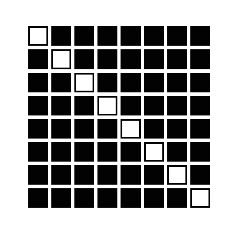
\includegraphics{pics/block_matrix.eps}
	\end{center}
	\caption{分块矩阵}
	\label{fig:blockmatrix}
\end{figure}
例如\figref{fig:blockmatrix}中的白色块代表的是满秩的块,黑色的部分代表的是缺秩的块矩阵。

那么这样的矩阵是否存在呢?答案是对于某些矩阵是存在的,特别是一些积分方程。快速多极算法就是基于这样的事实构造出来的.

例如:二维位势问题的核函数
\begin{equation}
	\varphi(x,y) = - \log (\|x-y\|)
\end{equation}
在复平面有,记$z = x, z_0 = y$有
\begin{equation}
	\varphi(x,y) = - \log (\|x-y\|) = Re (-\log(z-z_0)),
\end{equation}
当$|z| > |z_0|$时,它存在以下的展开式
\begin{equation}
	\log(z-z_0) = \log(z) - \sum_{k=1}^{\infty} \frac{a_k}{z^k}.
	\label{eq_expan}
\end{equation}
\begin{remark}
	上式说明$z$不在$z_0$附近的时候,截断上式就可以得到一个退化核近似。
\end{remark}

\subsubsection{多层结构}
前一节讲到分块矩阵的快速算法是由于矩阵的某些块不是满秩矩阵,非满秩矩阵的计算可以采用前述算法快速计算,满秩矩阵的计算则要全部计算,一个自然的想法就是这样的非满秩块矩阵越多越好,满秩矩阵越少越好。采用如下图一样的划分。
\begin{figure}[htbp]
	\begin{center}
		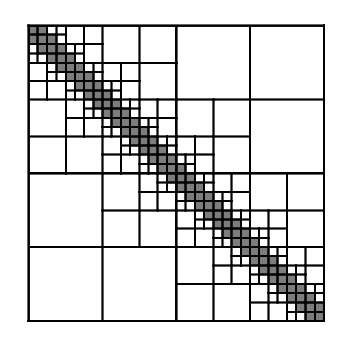
\includegraphics{pics/adaptive_matrix.eps}
	\end{center}
	\caption{多层矩阵结构划分}
	\label{fig:muli_matrix}
\end{figure}

灰色部分是满秩矩阵块,白色部分是非满秩矩阵块,采用这样的划分就可以很好地采用近似算法进行计算。直接计算的部分集中在对角线上,计算量较小。

快速多极算法也是这样的思想,首先将要求和的点按距离远近分组,二维的情形采用四叉树的结构。如下图所示结构

\begin{figure}[htbp]
	\begin{center}
		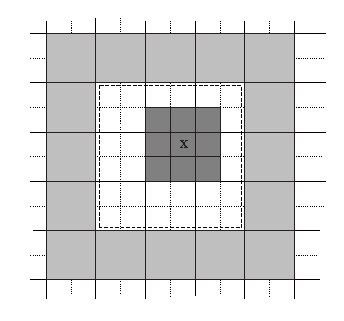
\includegraphics{pics/cluster.eps}
	\end{center}
	\caption{节点分组}
	\label{fig:cluster}
\end{figure}

由四叉树建立的过程,首先计算一个包含所有节点的正方形,称这个方形为四叉树的根结点,将正方形一分为四,称这四个方形为根结点的子节点,根结点为这四个子节点的父节点,若某一个子节点中的点的数目大于预设值,那么将该节点继续四分,依照样的法则直到树节点中的点的数目小于预设值。\footnote{这里可以写一个算法环境}

\begin{definition}
	邻接结点:与中心结点至少共有一个角点的树节点称为中心结点的邻接单元,如\figref{fignodetype}中淡蓝色所示; 
\end{definition}

\begin{definition}
	交互结点:若该树结点的父节点与中心结点的父节点互为邻接结点,并且不与中心结点的邻接,则称该节点为交互节点,如\figref{fignodetype}中黄色所示;
\end{definition}

\begin{definition}
	远程结点:既不是交互结点,也不是邻接结点的树结点,如\figref{fignodetype}中白色所示;
\end{definition}
\begin{figure}[htbp]
	\begin{center}
		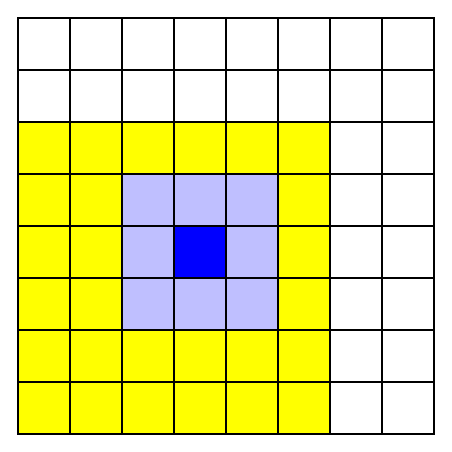
\includegraphics[width=0.4\textwidth]{pics/nabor.eps}
	\end{center}
	\caption{邻接结点,交互结点,远程结点}
	\label{fignodetype}
\end{figure}
单元的边长是$h$的话,如\figref{fig:cluster}所示,以$x$单元为中心展开的话,x中的点$x^*$到$x$树单元中点$x^*$的距离为$|x - x^*| < h$,而浅灰色树单元中的点到$x^*$的距离为$|y - x^*| > 2h$

对于二维位势问题,采用这样的划分,在同一层次上的树节点的非邻接节点上都满足公式\eqref{eq_expan},因此可以使用低秩近似,再下一层,中心节点的交互单元也满足\eqref{eq_expan},因此采用这样的结构可以利用原有的展开式进行矩阵的低秩近似。

\subsubsection{系数传递}
矩阵向量乘积的计算可以看作是分布在空间上的点两两相互作用,如\figref{fig:coefpass}左图所示,可见需要传递的信息是很多的,能否通过像\figref{fig:coefpass}右图所示的方式来传递系数呢?这样的传递方式显然更加的有效。
\begin{figure}[htbp]
	\begin{center}
		\includegraphics{pics/coef_passing.eps}
	\end{center}
	\caption{系数传递}
	\label{fig:coefpass}
\end{figure}
注意到简化算法中的系数$A_K$只与源点有关,$A_k$的计算是将源点的加起来,然后通过$A_k$计算位势。在这样的过程中,系数$A_K$就是一个传递的系数。

但是对于有奇异性的核函数,不能直接是使用需要通过多个传递系数,如\figref{fig:mulitipole}所示。同样也可以将场点分组起来。
\begin{figure}[htbp]
	\begin{center}
		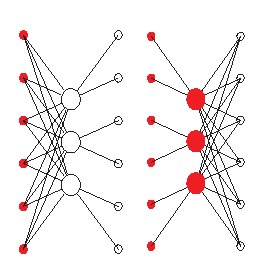
\includegraphics{pics/mulitipole.eps}
	\end{center}
	\caption{多组系数,奇异核}
	\label{fig:mulitipole}
\end{figure}

多极算法采用的是更加有效的传递过程,如下图所示,


\begin{figure}[htbp]
	\begin{center}
		\subfigure[]{
		\includegraphics{pics/single_level.eps}
		\label{fig:sfmm}
		}
		\subfigure[]{
		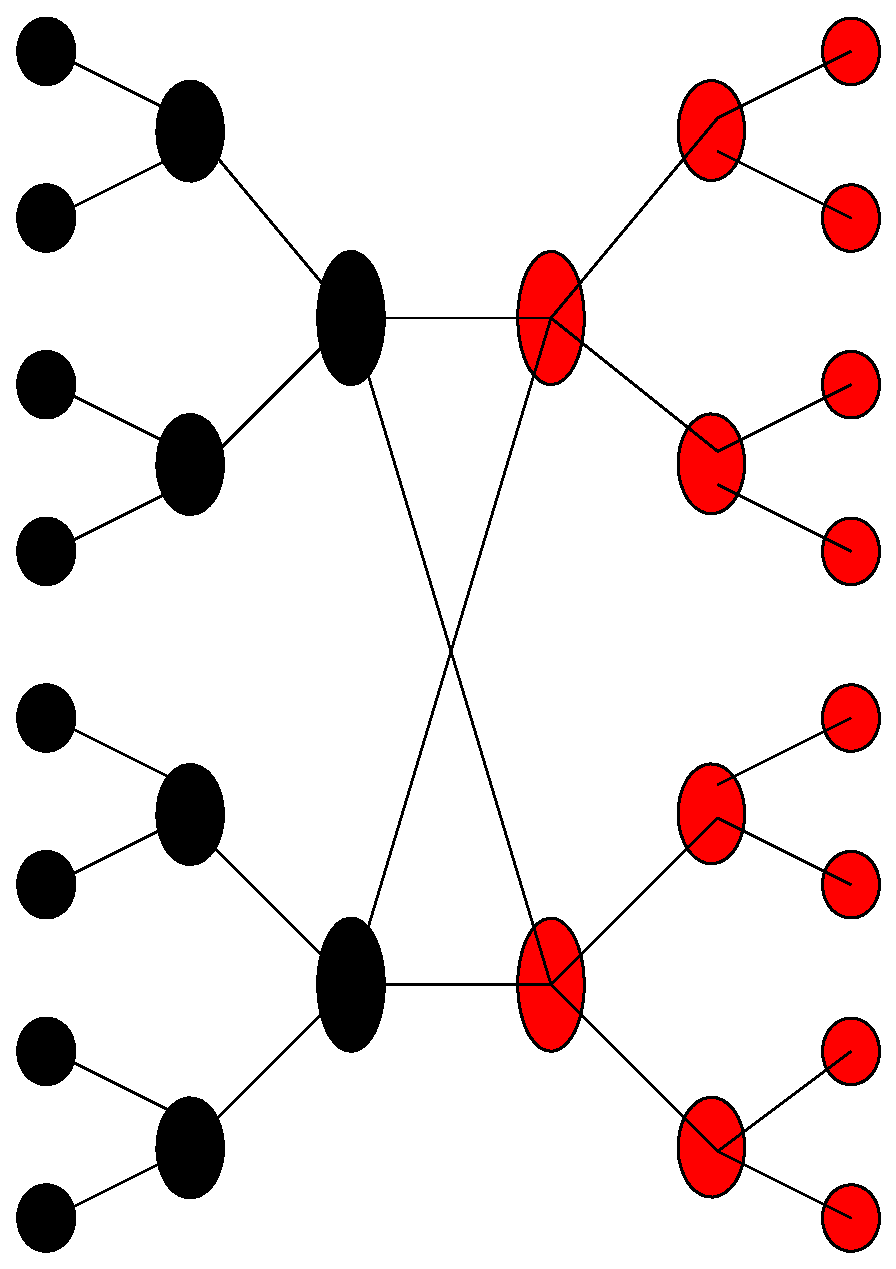
\includegraphics[width=0.15\textwidth]{pics/mulilevel.eps}
		%\caption{多层FMM}
		\label{fig:mfmm}
	}
		\caption{单层FMM和多层FMM}
\end{center}
\end{figure}


\section{积分算子的低秩近似}

假设$\Omega$是$R^d$的一个子流形或子区域,考虑如下的一个Fredholm积分算子,
\begin{equation}
	\mathcal{G}[u](x)= \int_{\Omega}g(x,y)u(y)dy,
\end{equation}
其中核函数$g(x,y)$是一个渐进光滑的,即存在常数$C_1,C_2$和奇异指数$s \in N$,使得下式成立,
\begin{equation}
	|\partial_{z}^{n}g(x,y)| \le C_1 (C_2 \| x-y \|)^{-n-s}n!
\end{equation}

\subsection{低秩近似}
考虑积分算子的Galerkin离散近似,其奇函数为$(\varphi_i)_{i \in I}$,则积分算子离散得到的矩阵为
\begin{equation}
	G_{i,j} = \int_{\Omega}\int_{\Omega}\varphi_i(x)g(x,y)\varphi_j(y) dxdy.
\end{equation}

若定义$r \times s \subseteq I \times I$是指标集的一个子集,并且定义相应的区域
\begin{equation}
	\tau := \cup_{i \in r} supp(\varphi_i), \sigma:=\cup_{i\in s}supp(\varphi_i)
\end{equation}
以及包含$\tau,\sigma$的平行盒子$B_{\tau},B_{\sigma}$.
若$dist(B_{\tau},B_{\sigma}) \ge 0$,则说明核函数$g|_{B_{\tau} \times B_{\sigma}}$是光滑的。
那么对于子矩阵$R:=K|_{r \times s}$能否找到一个近似矩阵$\hat{R}$.使得在某种意义下,矩阵的的近似
误差与离散误差是同一个量级的?
$\|R - \hat{R}\|$
如何能得到这样的一个结论?



\newpage
%% list references if any.
\putbib[20131020anarticle]
\newpage
	
